\documentclass[a4paper,12pt]{article}
\usepackage{graphicx}
\usepackage[a4paper, top=0cm, bottom=2cm, left=2cm, right=2cm]{geometry} % Ajuste les marges
\usepackage{xcolor} % Pour ajouter des couleurs
\usepackage{hyperref} % Pour avoir des références colorées si nécessaire
\usepackage{eso-pic} % Pour ajouter des éléments en arrière-plan

\usepackage[french]{babel}
\usepackage[T1]{fontenc}
\usepackage{mathrsfs}
\usepackage{amsmath}
\usepackage{amsfonts}
\usepackage{amssymb}
\usepackage{tkz-tab}

\usepackage{tikz}
\usetikzlibrary{arrows, shapes.geometric, fit}
\newcounter{correction} % Compteur pour les questions

% Définir la commande pour afficher une question numérotée
\newcommand{\question}{%
  \refstepcounter{correction}%
  \textbf{\textcolor{black}{Question \thecorrection (1 point) :}} \ignorespaces
}
% Commande pour ajouter du texte en arrière-plan
\AddToShipoutPicture{
    \AtTextCenter{%
        \makebox[0pt]{\rotatebox{80}{\textcolor[gray]{0.9}{\fontsize{10cm}{10cm}\selectfont PGB}}}
    }
}

\begin{document}
\hrule % Barre horizontale
% En-tête
\begin{center}
    \begin{tabular}{@{} p{5cm} p{5cm} p{5cm} @{}} % 3 colonnes avec largeurs fixées
        Lycée Dindéfélo & \quad\quad Test 10 & 12 Mars 2024 \\
    \end{tabular}
    \\[-0.01cm] % Ajuster l'espace vertical entre le tableau et la barre
    \hrule % Barre horizontale
\end{center}
\begin{center}
    \textbf{\Large Étude graphique} \\[0.2cm]
    \textbf{\large Professeur : M. BA} \\[0.2cm]
    \textbf{Classe : Terminale S2} \\[0.2cm]
    \textbf{\small Durée : 10 minutes} \\[0.2cm]
    \textbf{\small Note :\quad\quad /5}
\end{center}

% Nom de l'élève
\textbf{\small Nom de l'élève :} \underline{\hspace{8cm}} \\[0.5cm]

\subsection*{\underline{Étude graphique}}
Soit $f$ une fonction dont la courbe représentative est donnée ci-dessous :
\begin{figure}[h]% Forcer l'image à cet endroit
\centering
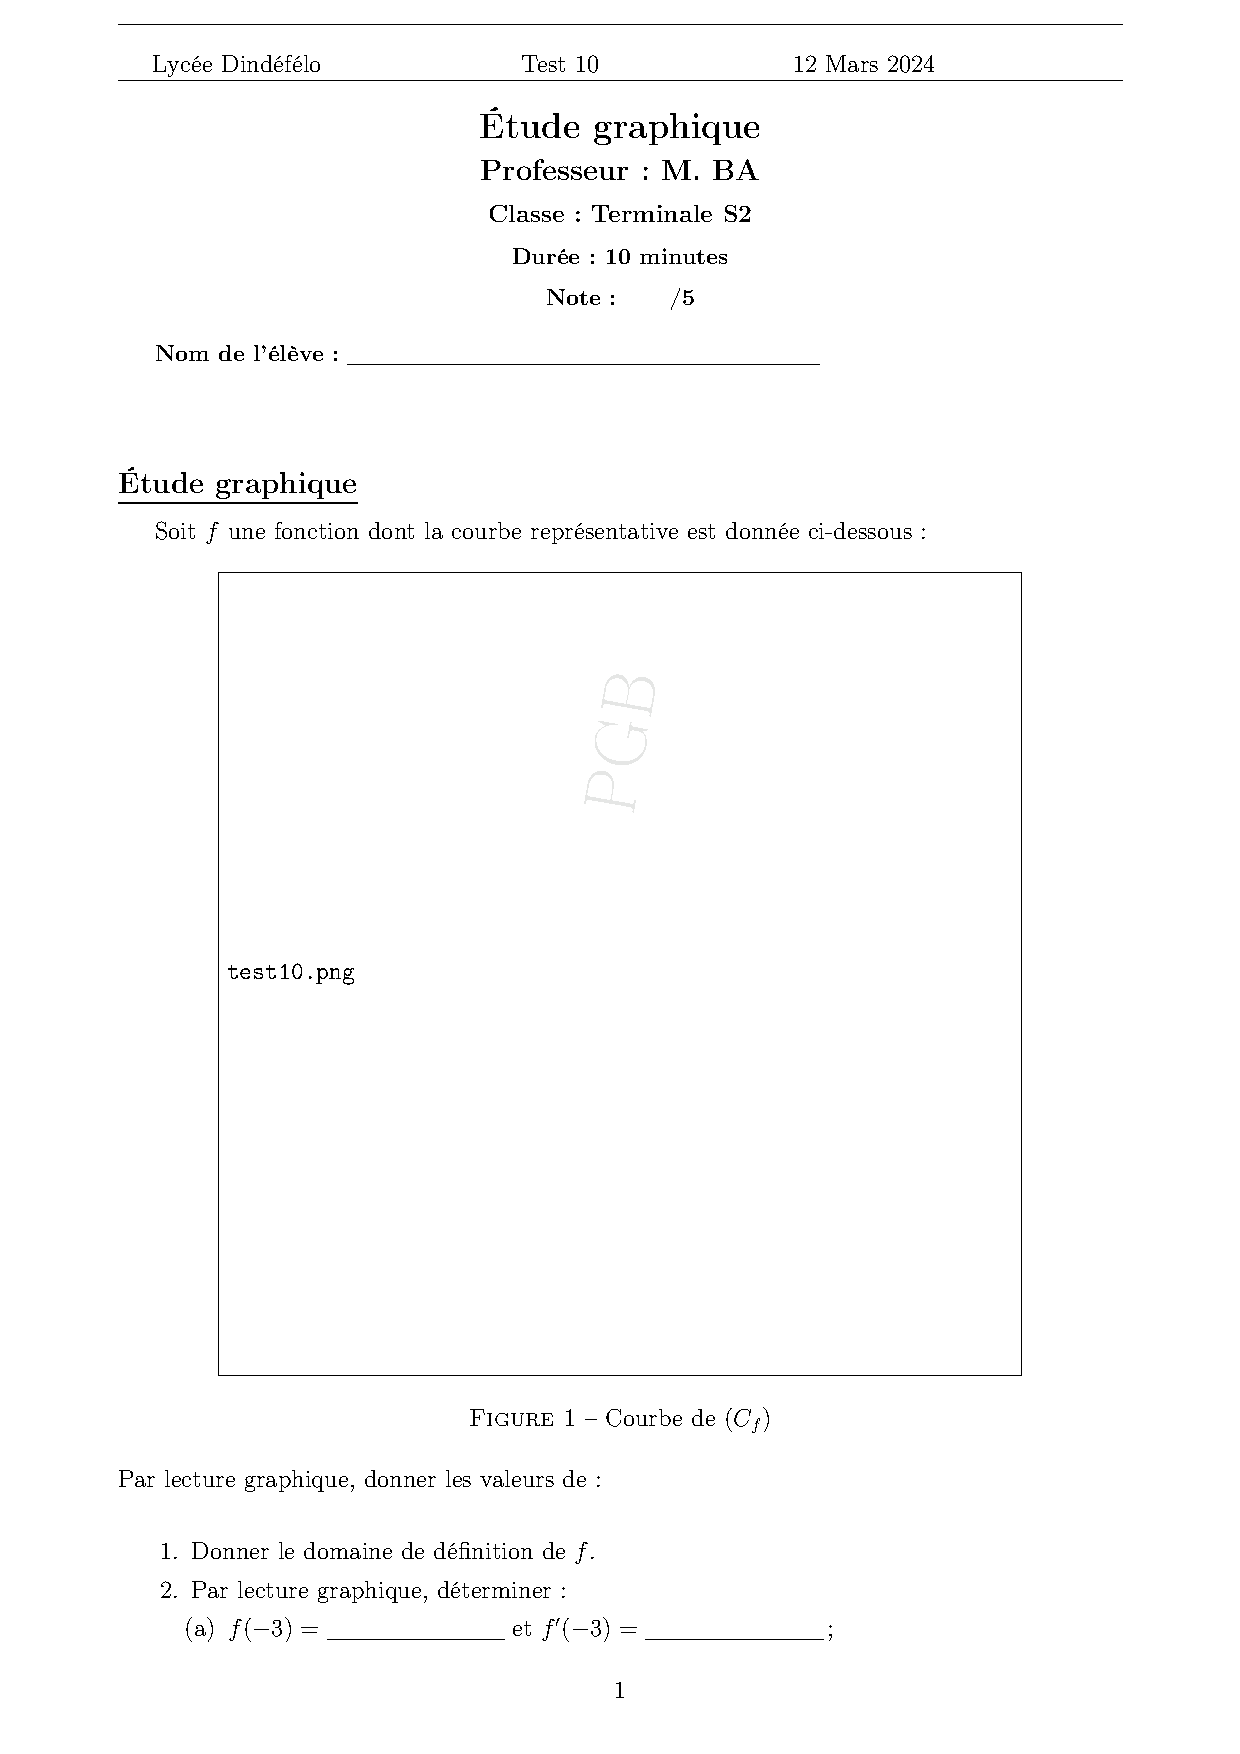
\includegraphics[width=0.8\textwidth]{test10.png}
\caption{Courbe de $(C_f)$}
\label{fig:monimage}
\end{figure}\\
Par lecture graphique, donner les valeurs de :\\

\begin{enumerate}
\item Donner le domaine de définition de $f$.
\item Par lecture graphique, déterminer :
\begin{enumerate}
\item $f(-3)=$ \underline{\hspace{3cm}} et $f'(-3)=$ \underline{\hspace{3cm}} ;
\item $f(0)=$ \underline{\hspace{3cm}} et $f'(0)=$ \underline{\hspace{3cm}} ;
\item $f(2)=$ \underline{\hspace{3cm}} et $f'(2)=$ \underline{\hspace{3cm}} ;
\item $f(5)=$ \underline{\hspace{3cm}} et $f'(5)=$ \underline{\hspace{3cm}}.
\end{enumerate}
\item Donner les limites suivantes de $f$ :
\begin{enumerate}
\item $\lim\limits_{x\to -\infty} f(x)=$ \underline{\hspace{3cm}} et $\lim\limits_{x\to +\infty} f(x)=$ \underline{\hspace{3cm}} ;
\item $\lim\limits_{x\to 0} f(x)=$ \underline{\hspace{3cm}} et $\lim\limits_{x\to -3} f(x)=$ \underline{\hspace{3cm}}.
\end{enumerate}
\item Donner le tableau de variation de $f$.
\end{enumerate}

\end{document}
